\documentclass[12pt, a4paper, titlepage, oneside]{book}
\usepackage[utf8]{inputenc}
\usepackage[italian]{babel} %set language = italian
\usepackage{pdfpages} %include function for pdf
\usepackage{mathptmx} %set font type = times 
\textheight24cm\topmargin0mm\headheight0mm\headsep6mm\oddsidemargin20pt\evensidemargin30pt %margin 
\linespread{1.2} %interlinea
\pagestyle{plain}
\usepackage{hyperref}

\usepackage[backend=biber,style=numeric,sorting=none]{biblatex} %bibliography
\usepackage{csquotes}
\addbibresource{bibliography.bib}

\usepackage{titlesec} %style chapter
\titleformat{\chapter}
  {\normalfont\LARGE\bfseries}{\thechapter}{1em}{}
\titlespacing*{\chapter}{0pt}{3.5ex plus 1ex minus .2ex}{2.3ex plus .2ex}

\usepackage{graphicx} %insert image
\graphicspath{ {./images/} }
\usepackage{wrapfig} %for wrap figures
\usepackage{graphicx} %for size figures
\usepackage{subcaption} %for position figures

\usepackage{listings} %for code format
\usepackage{xcolor}
\definecolor{mGreen}{rgb}{0,0.6,0}
\definecolor{mGray}{rgb}{0.5,0.5,0.5}
\definecolor{mPurple}{rgb}{0.58,0,0.82}
\definecolor{backgroundColour}{rgb}{0.95,0.95,0.92}
\lstdefinestyle{CStyle}{
    backgroundcolor=\color{backgroundColour},   
    commentstyle=\color{mGreen},
    keywordstyle=\color{magenta},
    numberstyle=\tiny\color{mGray},
    stringstyle=\color{mPurple},
    basicstyle=\footnotesize,
    breakatwhitespace=false,         
    breaklines=true,                 
    captionpos=b,                    
    keepspaces=true,                 
    numbers=left,                    
    numbersep=5pt,                  
    showspaces=false,                
    showstringspaces=false,
    showtabs=false,                  
    tabsize=2,
    language=C
}

\begin{document}
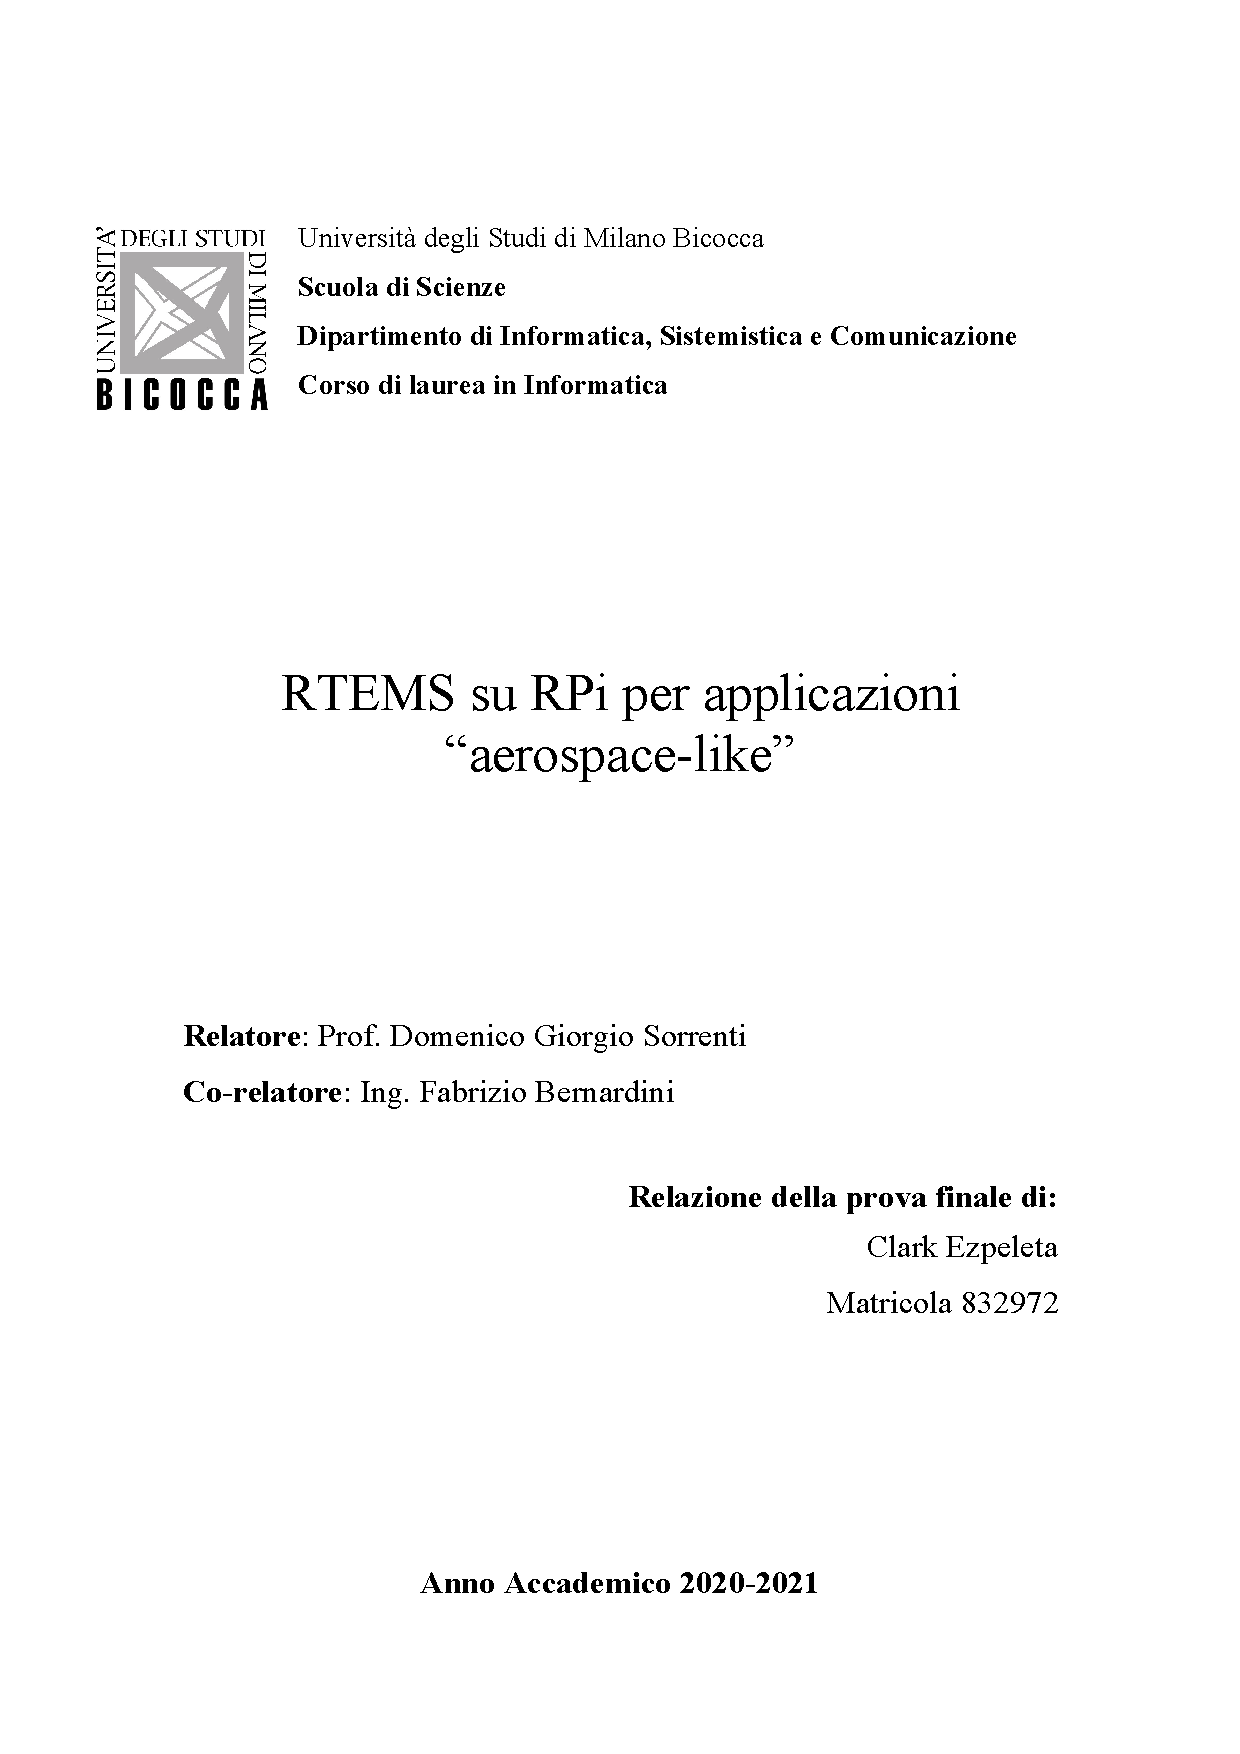
\includepdf[pages={1}]{Frontespizio_Ezpeleta.pdf}
\tableofcontents
\setcounter{page}{0}
\begin{flushleft}
\chapter*{Introduzione}
\setcounter{page}{1}

\addcontentsline{toc}{chapter}{Introduzione} 
Il lavoro che ho svolto ha due obiettivi principali: il 'porting' di RTEMS su Raspberry Pi e la creazione di applicativi RTEMS per validare il corretto funzionamento delle interfacce GPIO, UART, I2C, SPI  e l'utilizzo degli interrupts tramite le API di RTEMS.\\
%Lo scopo del mio lavoro consiste nel 'porting' di RTEMS su Raspberry Pi e nella creazione di applicativi RTEMS  per testare il funzionamento delle interfacce GPIO, UART, I2C, SPI e l'utilizzo degli interrupts.

Per poter svolgere il 'porting' ho fatto riferimento al RTEMS User Manual\cite{rtemsUM}, per comprendere meglio i concetti di RSB(RTEMS Source Builder) e BSP (board support packages), 
ed ho utilizzato la guida fornita da ing. Basile \cite{giorgio}, di BIS-Italia, che raccoglie tutti i passaggi esposti sul blog di Alan Tech per il 'porting' della versione 4.11.\\
%ed ho utilizzato la guida fornita da AlanC trovata sul suo blog \cite{alanT} in cui viene descritto il porting per la versione 4.11.\\
%Purtroppo la guida non è totalmente corretta, poiché datata a Marzo 2013 ed è stata scritta per la versione di RTEMS precedente a quella che ho utilizzato, cioè la 5.1 che è la più recente e stabile. \\
Purtroppo i passaggi illustrati sul blog non sono totalmente corretti, poiché sono per il 'porting' della versione di RTEMS precedente a quella che ho utilizzato, cioè la 5.1 che è la più recente e stabile.
Il 'porting' può essere definito corretto se alla fine della procedura si riesce a caricare uno degli applicativi di test forniti da RTEMS, su Raspberry Pi senza errori.\\
Dopo aver effettuato correttamente il 'porting', ho creato una guida in italiano  che raggruppa tutti i passaggi effettuati integrando le correzioni necessarie, ed è stata corretta anche la guida di ing. Basile \cite{giorgio5}.\\
Dopo aver impostato l'ambiente di lavoro ho iniziato a creare gli applicativi RTEMS da eseguire sulla Raspberry Pi.\\
Per poter creare gli applicativi RTEMS ho dovuto  familiarizzare con il linguaggio C, leggere l'RTEMS Classic API Guide \cite{rtemsCAG} ed analizzare i codici sorgente di esempio trovati nel git repository di asuol\cite{asuol} per poter comprendere l'utilizzo delle API. \\
Tutto il lavoro è stato eseguito in modalità "smart-working", per questo motivo mi è stata messa a disposizione da BIS-Italia la scheda Raspberry Pi 3B+ per poter effettuare l'attività. Microchip Technologies ha gentilmente offerto dei componenti aggiuntivi utili per gli applicativi RTEMS di test dell'interfaccia I2C e SPI.\\
Oltre all'attività software ho dovuto eseguire una piccola attività hardware, cioè creare dei circuiti saldando i vari componenti e utilizzando la breadboard in modo da poterli collegare alla Raspberry Pi, per fare ciò ho seguito gli schemi elettrici che mi ha inviato ing. Bernardini e ho letto i datasheet dei componenti dell'interfaccia I2C \cite{microchipMCP3425} \cite{microchipADC} e  SPI \cite{microchipMCP4822} \cite{microchipMSOP10-8} in modo da comprendere il loro funzionamento e poter creare i driver.\\

Premesso tutto ciò ho suddiviso la mia relazione nei seguenti capitoli:

\begin{itemize}
    \item \textbf{Capitolo 1} - in questo capitolo vengono descritte le principali tecnologie utilizzate durante il mio lavoro. Innanzitutto viene descritto RTEMS che è il sistema operativo su cui si basa tutta l'attività, dopodiché viene  descritta la Raspberry Pi su cui verranno eseguiti gli applicativi RTEMS, ed infine viene descritto Eclipse che è l'IDE utilizzato per creare gli applicativi.
    \item \textbf{Capitolo 2} - in questo capitolo viene descritta tutta l'attività di 'porting' e la definizione della toolchain per poter realizzare applicativi RTEMS. Vengono esposte tutte le problematiche rilevate e le loro soluzioni. 
    \item \textbf{Capitolo 3} - in questo capitolo vengono descritti le API che RTEMS ha a disposizione, la loro struttura e in che modo li ho testati e per quali motivi si è scelto di testarli.
    \item \textbf{Capitolo 4} - in questo capitolo viene descritta l'attività software che si basa sulla creazione degli applicativi RTEMS per testare il corretto funzionamento delle API di RTEMS. Viene esposto anche una descrizione dei componenti aggiuntivi offerti da Microchip di cui ho creato i driver per poterli utilizzare con RTEMS.
    \item \textbf{Capitolo 5} - in questo capitolo viene descritto ciò che si è raggiunto e la possibile estensione del mio lavoro.
\end{itemize} 

\chapter{Tecnologie}
\section{RTEMS}
\begin{figure}[h]
    \centering
    
\includegraphics[scale = 2]{rtemslogo.png}
\end{figure}
RTEMS sta per\textbf{ Real-Time Executive MultiProcessor System} ed è un sistema operativo real-time (RTOS) general purpose open source (licenza GPL 2.0 modificata) progettato e gestito da OAR Corporation. Il suo sviluppo iniziò nella fine degli anni 80 utilizzando i linguaggi Ada e C, e venne usato inizialmente per scopi militari, invece le prime versioni utilizzabili sono state rese open-souce su server ftp nel 1994.\\
Attualmente viene utilizzato in molti settori tra cui quello aerospaziale, infatti è stato utilizzato in alcune missioni spaziali sia a livello di on-board computer che come computer embedded in altre attività di volo
%ad esempio sul MRO (Mars Reconnaissance Orbiter) è in esecuzione un applicativo RTEMS che controlla l' Electra UHT Transceiver (EUT) che serve per la comunicazione tra Marte e la Terra . \\
RTEMS è  stato\textbf{ validato dall'ESA}, European Space Agency, ciò vuol dire che sono stati scritti dei programmi che riproducono gli scenari critici (ad esempio la gestione di molti dispositivi oppure la gestione e l'esecuzione concorrente dei task), e sono stati eseguiti sul sistema operativo per poter verificare il suo corretto funzionamento in quei casi. La validazione viene tutt'ora aggiornata poiché è un sistema operativo che è in continua evoluzione e avrà più funzionalità con il passare del tempo.\\
\textbf{RTEMS} non è un sistema operativo a sé stante, usato per caricare altri programmi, ma \textbf{è un executive} che viene compilato con l'applicazione in un unico codice monolitico da eseguire.

\newpage
RTEMS può essere visto come un insieme di direttive raggruppate in una serie di \textbf{manager}, che si occupano di varie funzionalità tra cui il controllo e la sincronizzazione dei task e processori, la gestione della memoria e la mutua esclusione. Invece la gestione dello scheduling, dispatching e object management sono forniti dal executive core.
\begin{figure} [h]
    \centering
    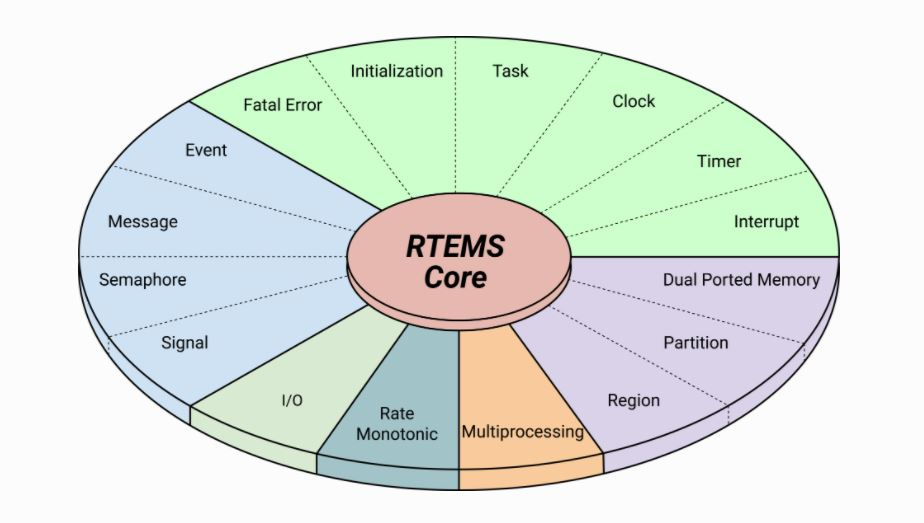
\includegraphics[scale = 0.80]{rtems_internal_architecture.JPG}
    \caption{Architettura RTEMS}
    \label{fig:my_label1}
\end{figure}

Utilizzando i managers di RTEMS lo sviluppatore può concentrarsi al solo sviluppo del applicativo e ciò riduce notevolmente il tempo di sviluppo.\\

La figura successiva mostra la logica di utilizzo di RTEMS.
\begin{figure}[ht]
    \centering
    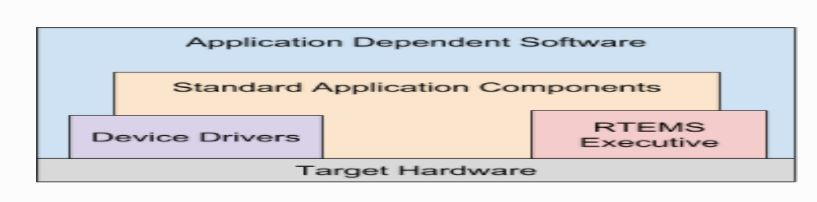
\includegraphics[scale = 0.80]{application_architecture.JPG}
    \caption{Struttura applicativo RTEMS}
    \label{fig:my_label2}
\end{figure}

Come si può notare RTEMS Executive è un intermediario tra il codice dell'applicativo e il target hardware, invece le dipendenze hardware con altri device sono localizzati nel livello 'device drivers'.
Il RTEMS I/O manager incorpora queste dipendenze hardware nel sistema mentre allo stesso momento fornisce all'application code l'accesso ad esse.
Queste dipendenze hardware sono isolate in specifiche \textbf{BSP}, Board Support Packages, per questo motivo il 'porting' di un applicativo RTMES su altri processori è semplice poiché basterebbe selezionare la BSP del microprocessore su cui si vuol eseguire l'applicativo e compilare con le sue librerie.\\
In questo modo durante lo sviluppo di un applicativo real-time si ha la totale indipendenza dall'architettura dei microprocessori. \\

E' disponibile il 'porting' di RTEMS su molte architetture CPU tra cui ARM, MIPS, LEON,ERC32 e i PowerPC; durante il mio lavoro ho trattato il 'porting' su architettura ARM utilizzando una Raspberry Pi 3B+.
\section{Raspberry Pi}
\begin{figure}[h]
    \centering
    
\includegraphics[scale = 0.70]{raspberrypiLogo.png}
\end{figure}
Raspberry Pi è una serie di computer a scheda singola sviluppata da Raspberry Pi Foundation in collaborazione con la Broadcom, in Inghilterra.\\
Originariamente è stato usato per insegnare le basi dell'informatica nelle scuole e nei paesi in via di sviluppo, ma attualmente grazie al suo basso prezzo viene usato anche nel settore della robotica, domotica e in molti altri.
Al momento sono state rilasciate quattro generazioni di Raspberry Pi, e tutti i modelli hanno un Broadcom SoC (System on Chip) con processore ARM integrato e on-chip GPU (Graphics Processing Unit).\\
Durante il mio lavoro viene usata la \textbf{Raspberry Pi 3B+} che utilizza il Broadcom BCM2837B0 SoC \cite{bcm2837} con processore Cortex-A53 (ARMv8) 64-bit 1.4Ghz.
\newpage
\begin{figure} [h]
    \centering
    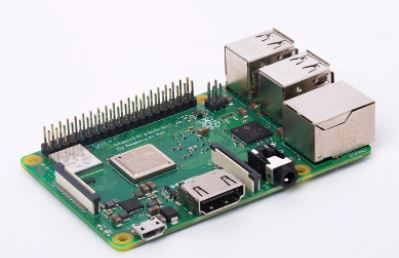
\includegraphics[scale = 1.25]{RPi3B.JPG}
    \caption{Scheda Raspberry Pi 3B+}
    \label{fig:RPI3B_laver}
\end{figure}
Tra le specifiche tecniche quelle che ci interessano maggiormente sono:
\begin{itemize}
    \item SDRAM LPDDR2 da 1GB.
    \item supporto per la micro SD.
    \item accesso a 40 GPIO.
\end{itemize}

Il 'bootloader' della Raspberry Pi 3B+ all'accensione della scheda cerca un file denominato "kernel7.img" per caricare il sistema operativo, ma noi vogliamo caricare degli eseguibili RTEMS e non un sistema operativo.
Per questo motivo la scheda SD deve essere gestita nel seguente modo:
\begin{enumerate}
    \item copiare il firmware di Raspberry Pi compatibile con RTEMS nella memoria SD.
    \item cancellare i file 'kernel*.img'. 
    \item compilare i sorgenti di un applicativo RTEMS in modo da ottenere il file con estensione'.img' 
    \item copiare l'eseguibile RTEMS nella memoria SD.
    \item impostare l'eseguibile RTEMS come kernel della scheda Raspberry Pi, modificando il file 'config.txt' aggiungendo il comando "kernel = nome\_eseguibile.img"
\end{enumerate}

In questo modo all'accensione della Raspberry Pi il 'bootloader' carica l'eseguibile RTEMS che prende il controllo della macchina.

\newpage
La figura successiva mostra tutti i pin GPIO che Raspberry Pi 3B+ ha a disposizione:
\begin{figure}[h]
    \centering
    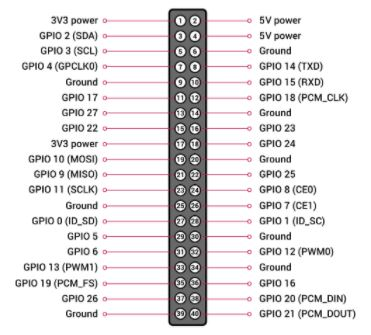
\includegraphics[scale = 1.50]{RPi3B_GPIO.JPG}
    \caption{Raspberry Pi 3B+ GPIO}
    \label{fig:RPi3B_GPIO}
\end{figure}

I livelli logici della scheda sono : alto se la tensione è pari a 3V3, basso se 0V; a questi livelli di solito corrispondono i valori binari 1 e 0.\\
I pin configurabili come input sono 3V3 'tolerant', quindi ricevono in input una tensione che va da 0v a 3V3, ed ogni pin ha una resistenza di pull-down o pull-up che è possibile impostare da software.
I pin configurabili come output possono dare una tensione da 0V a 3V3.\\
Infine alcuni pin possono essere utilizzati anche per gestire altre interfacce come l'I2C, UART, SPI.
\newpage
\section{Eclipse}
Eclipse è un IDE open source rilasciato con licenza EPL (Eclipse Public License) creato da IBM usato principalmente per la programmazione in Java ma grazie a vari plugin può essere usato per altri linguaggi di programmazione come C, C++, COBOL, Python e molti altri. \\
L'ambiente di sviluppo Eclipse include l'Eclipse Java development tools per Java, e l'Eclipse CDT per C/C++. \\
Per utilizzare RTEMS gcc cross compiler su Eclipse C, bisogna installare il plugin di RTEMS e settare le variabili di ambiente.
\begin{figure} [h]
    \centering
    \includegraphics[height = 135mm, width = 160mm ]{eclipse-i2c.png}
    \caption{Schermata Eclipse del programma I2C }
    \label{fig:eclips-i2c}
\end{figure}
\chapter{Porting di RTEMS su Raspberry Pi }

L'attività di 'porting' è la prima fase del lavoro e consiste in:
\begin{enumerate}
    \item Installazione dalla tool-suite sul computer host, dove vengono creati gli applicativi RTEMS.
    \item Verifica del corretto funzionamento della tool-suite, eseguendo i programmi di test su Raspberry Pi
    \item Configurazione del IDE Eclipse C, per la creazione di eseguibili RTEMS
    \item Provare a compilare e eseguire i programmi sia da terminale, e sia da Eclipse C
\end{enumerate}
Per svolgere tutta la procedura mi sono munito di un computer con sistema operativo Ubuntu, una scheda Raspberry Pi 3B+, una micro SD, e convertitore TTL USB.\\
%Tutta la procedura viene effettuata tramite comandi eseguiti su terminale.

RTEMS in sé è complesso per questo il team di RTEMS ci fornisce "l'ecosistema di RTEMS" che è una collezione di strumenti, packages, codici sorgente e documentazione, utile per definire come sviluppare, mantenere e usare RTEMS.\\
Durante il 'porting' ho utilizzato due importanti strumenti che fanno parte dell'ecosistema RTEMS, e sono :
\begin{itemize}
    \item\textbf{ RTEMS RSB }= l'RTEMS Source Builder è tool molto utile per compilare e fare la 'build' dei moduli di RTEMS e delle BSP 
    \item\textbf{ BSP raspberrypi }= la Build Support Package è il codice di supporto, che contiene le librerie di RTEMS per una specifica scheda (ad esempio la BSP raspberrypi viene usata per la Raspberry Pi 3B+)
\end{itemize}
L'installazione della tool-suite e BSP viene fatta tutta tramite comandi su terminale, non esiste un eseguibile .exe, ma viene usato il RTEMS RSB. Ci sono due requisiti necessari da rispettare e sono, avere installato Git per scaricare il codice sorgente di RTEMS, ed essere in grado di compilare i programmi C/C++ e Python poiché molti moduli della tool-suite sono scritti con questi linguaggi.\\
La versione di cui bisogna effettuare il porting è la \textbf{5.1} che è la più recente e stabile, anche se ciò ha dato problemi durante l'installazione perché la guida a cui facevo riferimento era per la versione precedente 4.1 rilasciata nel 2015, e veniva clonato il ramo main dove attualmente è presente una versione ancora in sviluppo.\\
Grazie all'aiuto dell'ing. Basile, siamo riusciti a capire che il problema stesse nel comando git.\\
La BSP raspberrypi da a disposizione dei programmi .exe da compilare e eseguire sulla scheda, in modo da verificare che l'installazione sia stata effettuata con successo.\\
Anche in questo caso ho avuto un problema riguardo la versione del firmware di Raspberry Pi copiato sulla scheda SD che non era compatibile con RTMES.\\
Per creare i file sorgenti per un applicativo RTEMS si possono usare un semplice editor di testo per poi compilarli tramite terminale, oppure utilizzare l'IDE Eclipse C/C++ per semplificare il processo.
Nel IDE ho dovuto installare un plugin per supportare RTEMS e impostare le variabili d'ambiente, in modo da 'puntare' al gcc cross compiler di RTEMS e la BSP corretta.\\
Come primo programma ho voluto creare un 'hello world', che manda tramite UART il messaggio su terminale. Durante la creazione ho avuto molti problemi dato che è stata la prima volta che creavo un applicativo RTEMS, infatti l'applicativo non mandava il log come ci si aspettava. Il problema risiedeva nella configurazione del sistema che inizializzava il driver del clock che per il nostro caso era inutile, e il driver della console errato.\\
Sono riuscito a compilare e 'buildare' correttamente i file sorgenti sia da terminale che da Eclipse, e ciò è verificato poiché il programma eseguito sulla Raspberry Pi non da errori.\\
A questo punto del lavoro ho creato una guida che espone tutti i passaggi corretti, cosicché qualunque utente voglia approcciarsi ad RTEMS su Raspberry Pi per la prima volta riesca a fare il porting e  senza dover cercare tra le tante fonti sparse su internet.\\
\textbf{La guida è disponibile in appendice alla relazione}
\chapter{Integrazione hardware e software}
%Qui ci va una descrizione delle varie interfacce disponibili in termini di drivers SW e come le abbiamo provate.
Effettuato il 'porting' sono passato all'attività software, cioè la creazione di RTEMS executive per testare il funzionamento delle RTEMS Classic API che sono le API per l'utilizzo delle interfacce. \\
\begin{figure} [h]
\centering
    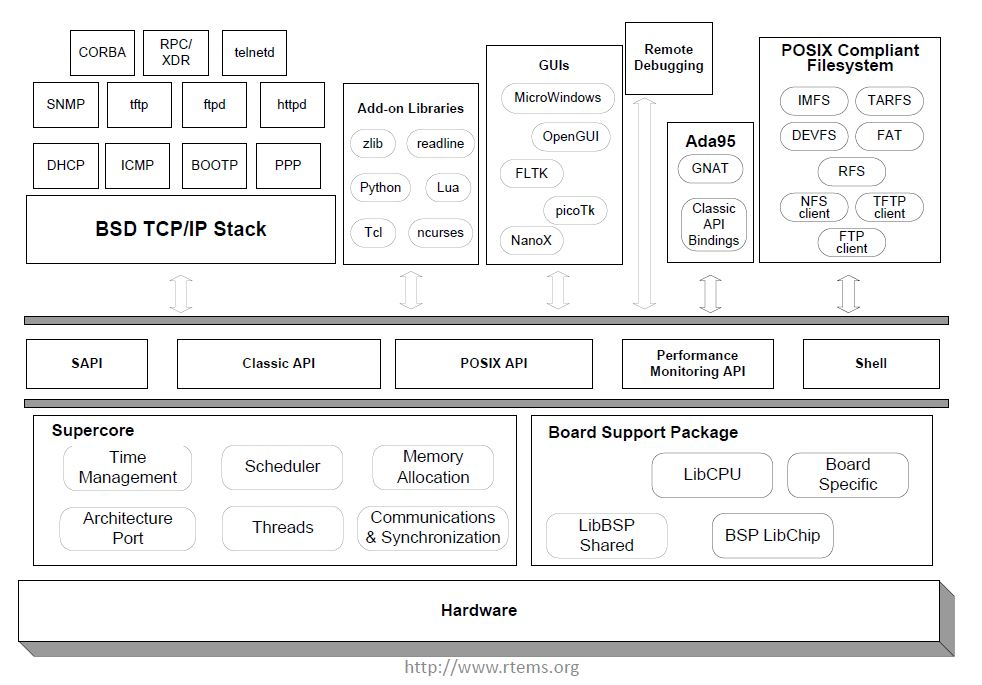
\includegraphics[scale = 0.80] {RTEMS_architecture.JPG}
    \caption{Architettura dettagliata sistema RTEMS}
    \label{fig:my_label3}
\end{figure}
Le interfacce che ci interessano validare sono:UART, GPIO, I2C, SPI.\\
La BSP dà a disposizione API e drivers per interfacciarci alle interfacce che ci interessano.\\
\newpage
La figura successiva mostra la struttura ed alcuni driver, file di configurazione e librerie presenti nella BSP utili per l'attività sperimentale:
\begin{figure} [h]
\centering
    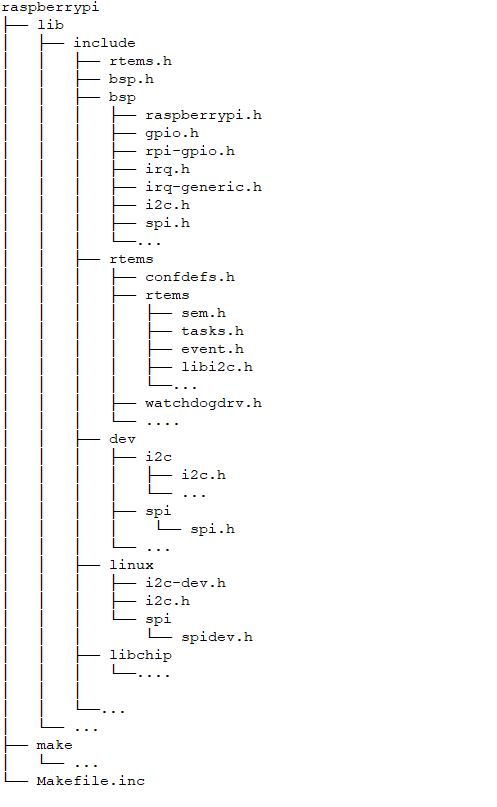
\includegraphics[scale = 1.0] {BSP_DIR_TREE.JPG}
    \caption{Struttura file BSP}
    \label{fig:Struttura cartelle BSP}
\end{figure}
\newpage
\begin{itemize}
    \item rtems.h = serve ad interfacciarsi ed includere tutte le RTEMS Classic API
    \item bsp.h = definisce le macro per la Rasperry Pi
    \item bsp/raspberrypi.h = definisce i registri della Raspberry Pi
    \item bsp/gpio.h = definisce le API per la gestione dei GPIO
    \item bsp/rpi-gpio.h = definisce le API per i GPIO specifiche per la Raspberry Pi
    \item bsp/irq.h = definisce le macro per utilizzare gli interrupt
    \item bsp/irq\_generic.h = definisce le API per la gestione degli interrupts
    \item bsp/i2c.h = definisce le API per I2C specifiche per la Raspberry Pi
    \item bsp/spi.h = definisce le API per SPI specifiche per la Raspberry Pi
    \item rtems/confdefs.h = serve a configurare il sistema su cui gira l'applicativo
    \item rtems/rtems/sem.h = definisce le API per gestire i semafori
    \item rtems/rtems/tasks.h = definisce le API per la gestione dei task
    \item rtems/rtems/event.h = definisce le API per la gestione degli eventi
    \item dev/i2c/i2c.h = definisce l'I2C driver framework ed è compatibile con la Linux I2C user-space API
    \item dev/spi/spi.h =  definisce il SPI driver framework ed è compatibile con la Linux SPI user-space API
   % \item linux/i2c-dev.h =
   %\item linux/i2c.h = 
   % \item linux/spi/spidev.h
   % \item libchip = cartella che contiene i device drivers, qui verranno inseriti i driver per i componenti MCP3425 e MCP4822
%TODO : to check
\end{itemize}
L'elenco sopra rappresenta è solo una\textbf{ piccola estrazione di cio che la BSP contiene} 
\chapter{Attività sperimentale}
\section{Obiettivi}
L'attività sperimentale consiste nella creazione di applicativi RTEMS per validare le API di RTEMS. Un API può essere considerata valida l'applicativo associato quando il comportamento del software è quello che ci aspettiamo e che venga fatto nell'arco temporale da noi definito.\\
\section{Test set-up}
Ogni programma di test creato implica un circuito elettrico differente costruito con jumper, breadboard, resistenze, condensatori, pulsanti, LED e schede aggiuntive mandate dalla Microchip su cui ho dovuto saldare cavetti e componenti per poterli utilizzare e collegare alla Raspberry Pi.\\

I componenti aggiuntivi sono :
\begin{itemize}
    \item MCP3425 SOT23-6 Evaluation Board  \cite{microchipMCP3425}: un evaluation board, con un ADC (Analog Digital Converter) MCP3425, controllato tramite protocollo I2C
    \item MSOP-10 and MSOP-8 Evaluation Board \cite{microchipMSOP10-8}: un evaluation board generica che serve per il collegamento del componente MCP4822 alla Raspberry Pi
    \item MCP4822 \cite{microchipMCP4822}: un DAC (Digital Analog Converter) controllato tramite protocollo SPI, montato sulla evaluation board sopracitata.
\end{itemize}
\newpage
Il componente \textbf{MCP3425} è un ADC, 'Analog Digital Converter', da 16 bit a canale singolo e vengono passati come input due tensioni ai pin $V_{IN}^+ $ e $ V_{IN}^-$ e viene restituito come output una tensione pari a $V_{IN}^+ - V_{IN}^- \times PGA$ ('Programmable Gain Amplifier') sul pin SDA (linea dati).\\ 
\begin{figure}[h]
\begin{subfigure}{0.5\textwidth}
    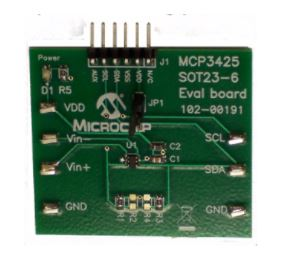
\includegraphics[width=0.9\linewidth, height=7cm]{MCP3425.JPG}
    \caption{MCP3425}
    \label{fig:MCP3425}
\end{subfigure}
\begin{subfigure}{0.5\textwidth}
    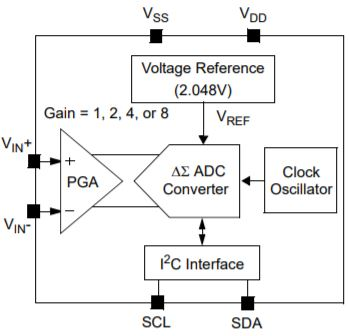
\includegraphics[width=0.9\linewidth, height=7cm]{images/MCP3425_block_diagram.JPG}
    \caption{schema a blocchi di MCP3425}
    \label{fig:MCP3425 block diagram}
\end{subfigure}
\end{figure}
Il componente ha la seguente configurazione predefinita:
\begin{itemize}
    \item Programmable Gain Amplifier(PGA) = 1
    \item Continuos Conversion
    \item Programmable Data Rate = 12 bit
\end{itemize}
Durante il lavoro viene utilizzata questa configurazione, ma nel caso si volesse cambiare la configurazione del componente, si può eseguire una scrittura di due byte dove il primo byte rappresenta l'indirizzo di periferica e il bit R/W (nel nostro caso è 11010000, dove R/W = 0 significa che stiamo eseguendo una scrittura) invece il secondo byte contiene i bit di configurazione\\
\begin{figure}[h]
    \centering
    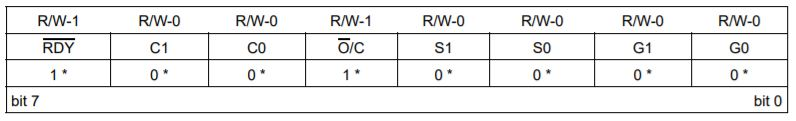
\includegraphics[scale = 0.9]{images/MCP3425_Configuration_register.JPG}
    \caption{Registro di configurazione MCP3425 con la configurazione preimpostata}
    \label{fig:CONFIG_REG_MCP3425}
\end{figure}
\newpage
\begin{figure}[h]
    \centering
    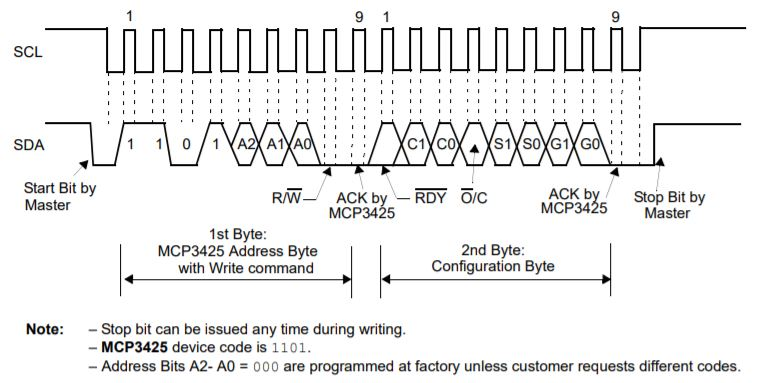
\includegraphics[scale = 1]{wrtie_configuration_MCP3425.JPG}
    \caption{Diagramma temporale scrittura su MCP3425}
    \label{fig:MCP3425_wrtie_conf}
\end{figure}
Su questo componente ci interessa effettuare la lettura della tensione in uscita che è rappresentata da due byte. Per eseguire la lettura bisogna seguire questi passaggi :
\begin{enumerate}
    \item mandare sul bus I2C l'indirizzo di periferica con R/W pari a 1
    \item lettura dei due byte
    \item conversione dei byte per avere il valore effettivo della tensione
\end{enumerate}

Dato che utilizziamo la configurazione preimpostata, abbiamo una conversione di 12 bit del dato, ciò comporta che nei due byte che riceviamo il dodicesimo bit rappresenta il segno e viene ripetuto fino al sedicesimo bit, quindi non dovremo considerare gli ultimi quattro bit.
Discorso analogo per la conversione in 14 bit e 16 bit.

\begin{figure}[h]
    \centering
    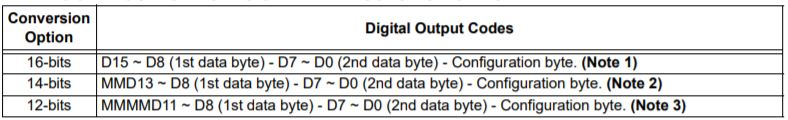
\includegraphics[scale = 1]{images/MCP3425_OUTPUT.JPG}
    \caption{Output MCP3425}
    \label{fig:MCP3425_wrtie_conf}
\end{figure}

\newpage
Il componente \textbf{MCP4822} è un DAC, 'Digital Analog Converter', da 12 bit a due canali e come input viene passato da programma 2 byte in cui viene rappresentato il dato da convertire e come output una tensione pari a $V_{OUT} = \frac{V_{ref} \times D_n}{2^n} \times G$ dove:
\begin{itemize}
    \item $V_{ref}$ = 2.048V
    \item $D_n$ = sono i bit che passo in input
    \item $n$ = è il numero dei bit, cioè 12
    \item $G$ = è il gain
\end{itemize}

%\begin{figure}[h]
%\begin{subfigure}{0.5\textwidth}
%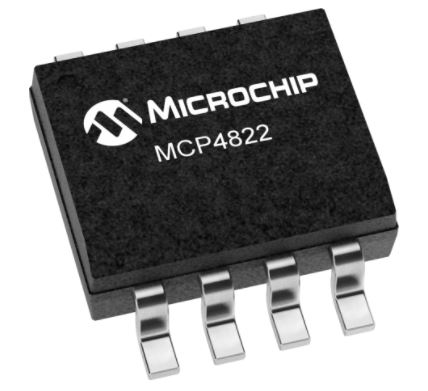
\includegraphics[width=0.8\linewidth, height=3cm]{images/MCP4822.JPG} 
%\caption{MCP4822}
%\label{fig:MCP4822}
%\end{subfigure}
%\begin{subfigure}{0.5\textwidth}
%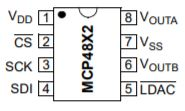
\includegraphics[width=0.7\linewidth, height=3cm]{images/MCP4822_pin.JPG}
%\caption{MCP4822 pin}
%\label{fig:MCP4822 pin}
%\end{subfigure}
%\end{figure}

\begin{figure} [h]
    \centering
    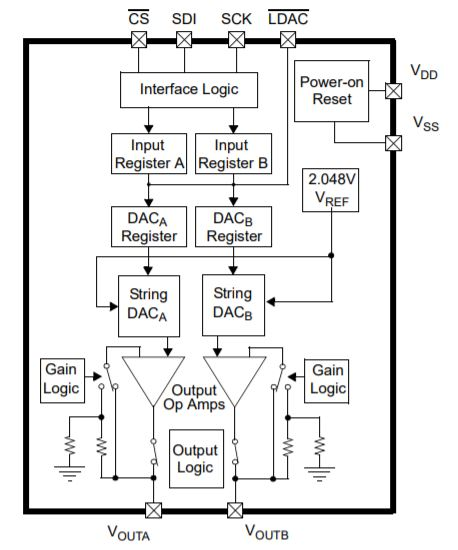
\includegraphics[scale = 1]{images/MCP4822_block_diagram.JPG}
    \caption{Schema a blocchi di MCP4822}
    \label{fig: MCP4822 BLOCK DIAGRAM}
\end{figure}

Il componente ha due canali e la comunicazione è unidirezionale, cioè non puo' essere eseguita una lettura ma solo la scrittura \\
\newpage
La scrittura viene effettuata mandando due byte di cui il primo è formato dai 4 bit di configurazione e gli ultimi 4 data bit, e il secondo è formato dai restanti data bit.\\
\begin{figure}[h]
    \centering
    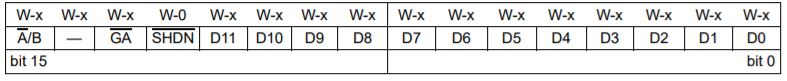
\includegraphics[scale = 1]{images/MCP4822_config_register.JPG}
    \caption{Registro di configurazione del MCP4822}
    \label{fig:MCP4822_CONF_REGISTER}
\end{figure}
\begin{figure}[h]
    \centering
    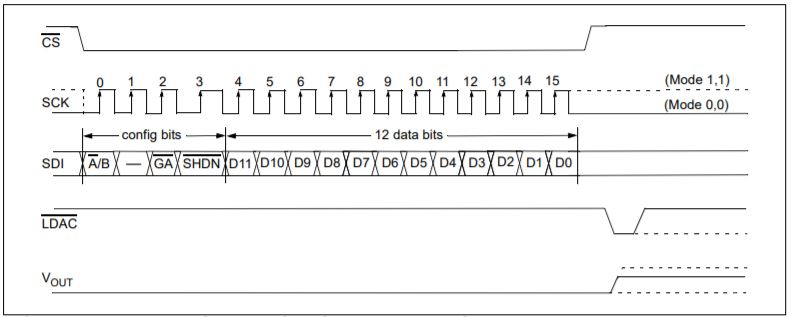
\includegraphics[scale = 1]{images/MCP4822_write_time_diagram.JPG}
    \caption{Diagramma temporale scrittura su MCP4822}
    \label{fig:MCP4822 TIME DIAGRAM}
\end{figure}

Effettuata la scrittura sul canale selezionato, il componente procede alla conversione del dato e restituisce la tensione. \\

\newpage
\section{Test application software}
La struttura principale che tutti i programmi seguono è la seguente:
\begin{itemize}
    \item init.c = è il file sorgente contenente la funzione Init che è il punto di partenza dell'eseguibile. E' come se fosse il metodo main in Java.
    \item init.h = è un file header che contiene tutte le direttive RTEMS per configurare il sistema
    \item task\_helper.c = è il file sorgente contenente la definizione dei task, le funzioni per la manipolazione delle variabili globali, le funzioni aggiuntive 
    \item task\_helper.h = è un file header che contiene tutte le dichiarazioni delle funzioni definite in task\_helper.c che si vogliono usare in init.c, ad esempio la definizione dei task.
\end{itemize}
La configurazione del sistema viene definita tramite le direttive RTEMS, si può definire una configurazione di base :
\begin{lstlisting}[style = CStyle]
#define CONFIGURE_APPLICATION_DOES_NOT_NEED_CLOCK_DRIVER
#define CONFIGURE_APPLICATION_NEEDS_SIMPLE_CONSOLE_DRIVER
#define CONFIGURE_UNLIMITED_OBJECTS
#define CONFIGURE_UNIFIED_WORK_AREAS
#define CONFIGURE_RTEMS_INIT_TASKS_TABLE
#define CONFIGURE_INIT

#include <rtems/confdefs.h>

\end{lstlisting}
\begin{itemize}
    \item CONFIGURE\_APPLICATION\_DOES\_NOT\_NEED\_CLOCK\_DRIVER : è necessario definirlo quando non si vuole utilizzare il driver del clock e del timer. Nel caso si voglia inizializzare il driver del clock bisogna utilizzare la direttiva CONFIGURE\_APPLICATION\_NEEDS\_CLOCK\_DRIVER, e impostare i microsecondi per tick con la direttiva CONFIGURE\_MICROSECONDS\_PER\_TICK.
    \item CONFIGURE\_APPLICATION\_NEEDS\_SIMPLE\_CONSOLE\_DRIVER: imposta il Simple Console Driver, in questo modo possiamo utilizzare la funzione "printf()" per la visualizzazione dei log.
    \item CONFIGURE\_UNLIMITED\_OBJECTS : con questa direttiva non si ha limiti di oggetti rtems, e non si ha il bisogno di gestire la RAM. Ovviamene questa direttiva non deve essere usata per applicativi da mandare in produzione, ma può essere usata durante la fase di test
    \item CONFIGURE\_UNIFIED\_WORK\_AREAS : da utilizzare quando la direttiva "CONFIGURE\_UNLIMITED\_OBJECTS" è definita poiché in questo modo viene utilizzata tutta la memoria disponibile, cioè  il  RTEMS Workspace e il C programm heap saranno in un unico pool di memoria.
    \item CONFIGURE\_RTEMS\_INIT\_TASKS\_TABLE : questa direttiva è necessaria per indicare che l'applicativo parte eseguendo il task Init che ha la priorità massima (1) e non è preemptive.
    \item CONFIGURE\_INIT : direttiva necessaria per far si che la libreria \textbf{rtems/confdefs.h} (che deve essere inclusa nel file header) istanzi la configurazione del sistema
\end{itemize}
Il primo programma di test che ho creato è quella per l'\textbf{interfaccia UART} e si tratta di un "hello world!". È stato il più semplice da creare, poiché durante il 'porting' è stato usato un programma di esempio simile per visualizzare i log di sistema. Dal codice sorgente dei programmi di esempio forniti da RTEMS, come quelli per il ticker.img,  si può ipotizzare correttamente che per far stampare un messaggio sulla console è sufficiente definire la direttiva di sistema 
\begin{lstlisting}[language = C]
#define CONFIGURE_APPLICATION_NEEDS_SIMPLE_CONSOLE_DRIVER 
\end{lstlisting} 
e usare le funzioni della libreria standard stdio.h \begin{lstlisting} [language = C]
printf("log");  fflush(stdout);
\end{lstlisting}
ed ho come risultato:
\begin{figure}[h]
    \centering
    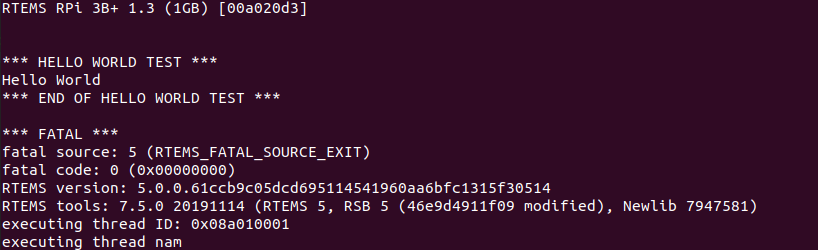
\includegraphics[scale = 0.5]{images/hello_world_log.png}
    \caption{Hello world log}
    \label{fig:hello_world_log}
\end{figure}

Il messaggio di errore su terminale è causato dalla funzione \textbf{'exit(n)'}, presente nel task Init per \textbf{terminare l'applicativo} con 'fatal code' uguale al parametro 'n'.
La funzione 'exit(n)' causa un messaggio di errore perché si prevede che un applicativo RTEMS sia sempre in esecuzione, e quindi il termine di esso per RTEMS è considerato un comportamento imprevisto.
Se non si vuole avere questo messaggio di errore bisogna inserire nel codice un ciclo infinito, in modo che il programma non termini.
%Senza la funzione 'exit(n)' avremmo il codice di errore uguale a 5 che corrisponde ad INTERNAL\_ERROR\_THREAD\_EXITTED poiché non essendoci altre funzioni o un ciclo infinito dopo la funzione 'printf(..)', il task Init termina . 
\newpage
L'\textbf{interfaccia GPIO }è stata testata con tre programmi per coprire le seguenti situazioni :
\begin{enumerate}
    \item accensione e spegnimento di un led ad intervalli di 1 secondo.
    \item alla pressione di un bottone si ha l'accensione o spegnimento di un led.
    \item alla pressione di un bottone, viene avviato un task.
\end{enumerate}

Il \textbf{primo programma} sui GPIO, il file init.c ha solo il task Init, dove è presente un ciclo infinito (while(1)) per il cambio di stato del LED e le API di RTEMS per la gestione del GPIO :
\begin{itemize}
    \item rtems\_gpio\_initialize() : inizializza le API dei GPIO
    \item rtems\_status\_code rtems\_gpio\_bsp\_select\_input(uint32\_t bank,uint32\_t pin,  void *bsp\_specific) : imposta il pin come input, discorso analogo l'output.
    \item uint32\_t rtems\_gpio\_bsp\_get\_value(uint32\_t bank, uint32\_t pin) : recupera il valore del pin
    \item rtems\_status\_code rtems\_gpio\_bsp\_clear(uint32\_t bank, uint32\_t pin) : imposta il valore del pin a 0
    \item rtems\_status\_code rtems\_gpio\_bsp\_set(uint32\_t bank, uint32\_t pin) : imposta il valore del pin a 1
\end{itemize}
\begin{lstlisting}[style = CStyle]
  ...
  rtems_interval  seconds = 1 * rtems_clock_get_ticks_per_second();
  rtems_gpio_initialize();
  rtems_gpio_bsp_select_input(0, pin, &bsp_spec);
  rtems_gpio_bsp_select_output(0, pin, &bsp_spec);
  while(1){
	  if(rtems_gpio_bsp_get_value(0, pin)){
		  rtems_gpio_bsp_clear(0,pin);
	  }else{
		  rtems_gpio_bsp_set(0,pin);
	  }
	  rtems_task_wake_after(seconds);
  }
...

\end{lstlisting}
%Nel file header init.h per la configurazione di sistema ho impostato i microsecondi per ogni tick a 1000000 che equivale a 1 secondo per ogni tick
\newpage
Il \textbf{secondo programma} sui GPIO ha come scopo validare anche la gestione degli interrupts. 
Ho dovuto creare un circuito elettrico per generare un interrupt tramite pulsante e vedere la gestione dallo stato di un LED.\\
\begin{figure}[h]
\begin{subfigure}{0.5\textwidth}
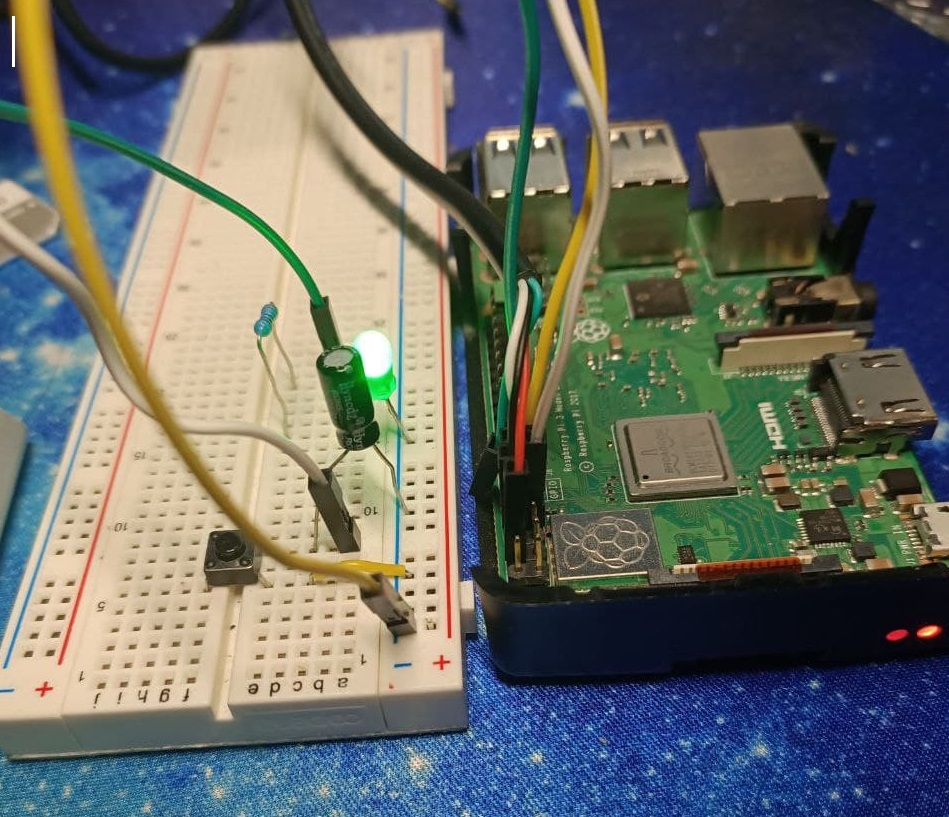
\includegraphics[width=1.2\linewidth, height=7cm]{images/Btn_switch_led_circuit_image.JPG}
\caption{Circuito con Raspberry Pi}
\label{fig:Circuito con Raspberry Pi}
\end{subfigure}
\begin{subfigure}{0.5\textwidth}
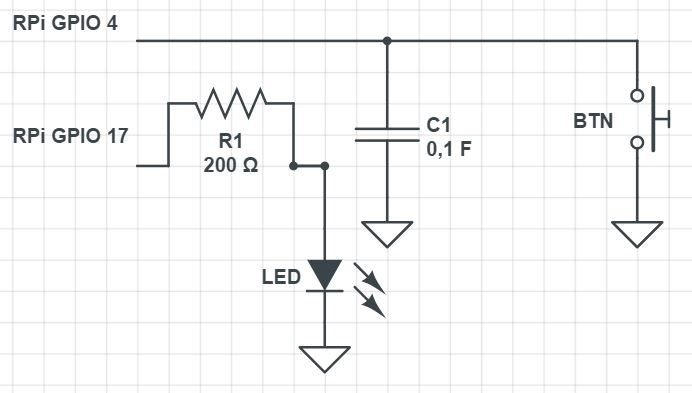
\includegraphics[width=1.2\linewidth, height=7cm]{images/Btn_switch_led_circuit_schema.JPG}
\caption{Schema elettrico del circuito}
\label{fig:Schema elettrico del circuito}
\end{subfigure}
\end{figure}
In questo programma si hanno due task, Init e ld\_switch.
Il task Init si occupa della configurazione dei GPIO e interrupts, creazione del task ld\_switch, creazione del semaforo e avvio del ld\_switch.
Il task ld\_switch è quello che esegue il cambio di stato del LED che dipende dallo stato del pulsante gestito da interrupt.
Per la configurazione degli interrupt ho utilizzato le API di RTEMS generiche :
\begin{itemize}
    \item rtems\_status\_code rtems\_gpio\_resistor\_mode(
  uint32\_t pin\_number,
   rtems\_gpio\_pull\_mode mode
) : imposta in pull-up o pull-down la resistenza del pin
    \item rtems\_status\_code rtems\_gpio\_enable\_interrupt(
  uint32\_t pin\_number,
  rtems\_gpio\_interrupt interrupt,
  rtems\_gpio\_handler\_flag flag,
  bool threaded\_handling,
  rtems\_gpio\_irq\_state (*handler) (void *arg),
  void *arg
) : abilita l'interrupt sul pin, e assegna l'handler già definito.
    \item rtems\_status\_code rtems\_gpio\_debounce\_switch(
  uint32\_t pin\_number,
  int ticks
) : imposta il tempo del debounce del pin. 
\end{itemize}
Tra l'handler dell'interrupt e il task ld\_switch si verifica il problema della gestione della \textbf{sezione critica} sulla variabile dello stato del pulsante, ciò è stata risolta utilizzando gli \textbf{eventi} e un \textbf{semaforo binario}.\\
Per utilizzare i semafori è necessario aggiungere una direttiva in più "CONFIGURE\_MAXIMUM\_SEMAPHORES " impostando il numero massimo di semafori consentiti, nel nostro caso 1.\\
Di seguito il codice in cui viene gestita la sezione critica
\begin{lstlisting}[style = CStyle]
...
rtems_gpio_irq_state btn_handler(void *arg) {
	sem_status = rtems_semaphore_obtain(sem_id,RTEMS_WAIT, RTEMS_NO_TIMEOUT);
	if(sem_status != RTEMS_SUCCESSFUL){
		print_to_console_error("rtems_sem_obt failed ", sem_status);
		exit(sem_status);
	}
	//send event to ld_switch task
	rtems_event_send(tid_1, RTEMS_EVENT_0);
	if(get_ld_status()){
		set_ld_status(false);
	}else{
		set_ld_status(true);
	}
	rtems_semaphore_release(sem_id);
	return IRQ_HANDLED;
}
rtems_task ld_switch(rtems_task_argument sec){
	print_to_console("initialized btn_polling_task \n");
	rtems_event_set event_out;
	while(1){
		//wait until btn_interrupt send event
		rtems_event_receive(RTEMS_EVENT_0, RTEMS_WAIT, RTEMS_NO_TIMEOUT, &event_out);
		//wait until btn_interrupt release semamphore
		sem_status = rtems_semaphore_obtain(sem_id, RTEMS_WAIT, RTEMS_NO_TIMEOUT);
		if(sem_status != RTEMS_SUCCESSFUL){
			print_to_console_error("rtems_sem_obt failed ", sem_status);
			exit(sem_status);
		}
		if(get_ld_status()){
			rtems_gpio_bsp_set(0, ld_pin);
			print_to_console("1");
		}else{
			rtems_gpio_bsp_clear(0, ld_pin);
			print_to_console("0");
		}
		rtems_semaphore_release(sem_id);
	}
}
\end{lstlisting}


%TODO: FINIRE o sistemare
%TODO: DESCRIZIONE DEL TERZO PROGRAMMA, DESCRIVENDO LA GESTIONE DEI TASK (STATO DEL TASK) \\
\newpage
Il \textbf{terzo programma} è composto da due task oltre il task Init:
\begin{itemize}
    \item \textbf{btn\_polling} : controlla la variabile di stato del pulsante, se risulta true (quindi è stato  premuto), allora viene avviato il task led\_blink
    \item \textbf{led\_blink} : accende o spegne 3 volte il LED con un intervallo di tempo di 1 secondo.
\end{itemize}
Il circuito elettrico è lo stesso del programma precedente.
Anche in questo programma è presente la sezione critica per la variabile di stato del pulsante, e viene gestita nello stesso modo.
In questo caso bisogna modificare lo stato dei task in modo da non farli interferire tra loro.\\
\begin{figure}[h]
    \centering
    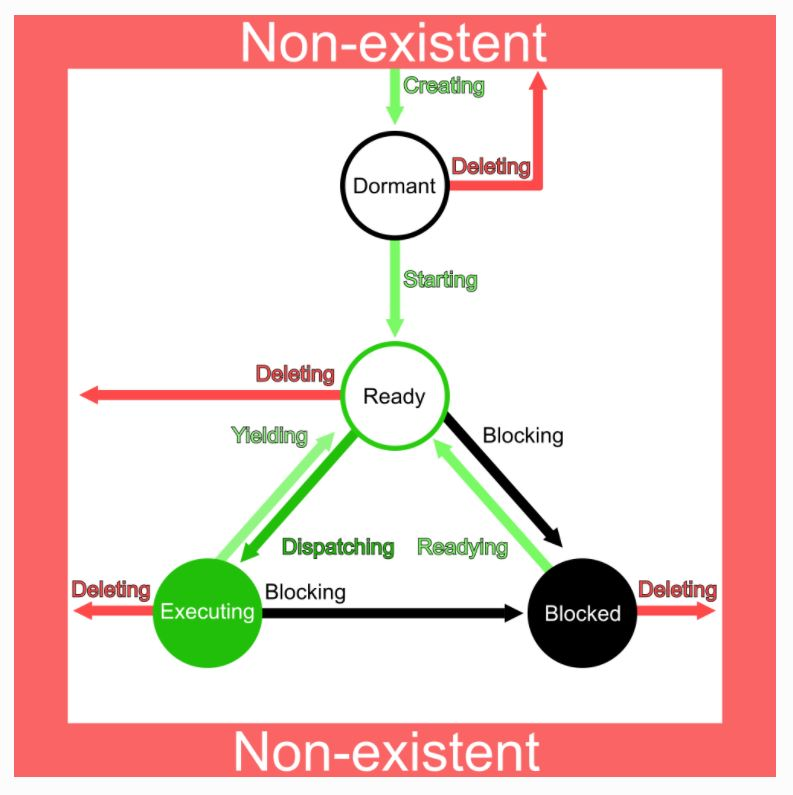
\includegraphics[scale = 0.5]{images/task_state.JPG}
    \caption{Stato dei task}
    \label{fig:Stato dei task}
\end{figure}
Il task Init dopo aver configurato l'applicativo e creato i task, avvia il task btn\_polling che passa dallo stato 'Ready' allo stato 'Executing'.
Il task btn\_polling quando riceve riceve l'evento dall'handler interrupt avvia il task ld\_blink cambiandogli stato da 'Ready' a 'Executing' con l' API rtems\_task\_restart(..) oppure rtems\_task\_start(..), ciò dipende se il task era in stato 'Blocked'. Inoltre viene cambiato lo stato del task btn\_polling in 'Blocked' con l'API rtems\_task\_suspend(..).\\
In questo modo rimane in esecuzione solo il task ld\_blink, che come ultime operazioni ha il  ripristino dell'esecuzione del task btn\_polling con l'API rtems\_task\_resume e quindi viene cambiato lo stato in 'Executing' e viene sospeso il task ld\_blink.\\
Seguendo questi passaggi rimane in esecuzione solo un task alla volta.
%Il task Init dopo aver configurato il sistema e creato i task, avvia il task btn\_polling.
\newpage
\begin{lstlisting}[style = CStyle]
...
rtems_task btn_task(rtems_task_argument sec){
	print_to_console("initialized btn_polling_task \n");
	rtems_event_set event_out;
	while(1){
		rtems_event_receive(RTEMS_EVENT_0, RTEMS_WAIT, RTEMS_NO_TIMEOUT, &event_out);
		sem_status = rtems_semaphore_obtain(sem_id, RTEMS_WAIT, RTEMS_NO_TIMEOUT);
			if(btn_status == true){
				status_1 = rtems_task_restart( tid_2, 0);
				if ( status_1 == RTEMS_INCORRECT_STATE ) {
					rtems_task_start(tid_2,ld_blink,0);
			   }else if (status_1 != RTEMS_SUCCESSFUL){
				   print_to_console_error("ld_blink_task start failed ", status_1);
			   }
				rtems_task_suspend(tid_1);
				btn_status = false;
			}
		rtems_semaphore_release(sem_id);
	}
}
rtems_task ld_blink(rtems_task_argument null){
	rtems_interval two_sec = 2 * rtems_clock_get_ticks_per_second();
	uint32_t count = 0;
	print_to_console("initialized ld_blink_task \n");
	while(count<4){
		if(rtems_gpio_bsp_get_value(0, ld_pin)){
			rtems_gpio_bsp_clear(0, ld_pin);
		}else{
			rtems_gpio_bsp_set(0, ld_pin);
			count++;
		}
		rtems_task_wake_after(two_sec);
	}
	btn_status=false;
	rtems_task_resume(tid_1);
	rtems_task_suspend(tid_2);
}
\end{lstlisting}
\newpage

%TODO : da controllare
L'interfaccia \textbf{I2C} è stata testata creando un programma che legge l'output del componente ADC che ,manipolandolo come indicato dal datasheet, da come risultato la tensione in entrata al ADC convertendo il dato da analogico a digitale. Poiché bisogna utilizzare un componente aggiuntivo, ho dovuto creare il driver associato.\\
Il driver è composto da due file sorgenti:
\begin{itemize}
    \item mcp3425.h = in questo file viene dichiarata la funzione int i2c\_dev\_register\_mcp3425(const char *bus\_path, const char *dev\_path, uint16\_t address); che serve per configurare il bus I2C ed associare il file in dev\_path all'indirizzo di periferica address.
    Questo file header deve essere inserito nella cartella libchip, che contiene tutti i file header dei driver .
    \item mcp3425.c =  in questo file viene definita la funzione i2c\_dev\_register\_mcp3425, e i comandi ioctl che verranno utilizzato nel programma.
\end{itemize}

La funzione i2c\_dev\_register\_mcp3425 è così definita:
\begin{lstlisting}[style = CStyle]
int i2c_dev_register_mcp3425(const char *bus_path, const char *dev_path, uint16_t address) {
  i2c_dev *dev;
  dev = i2c_dev_alloc_and_init(sizeof(*dev), bus_path, address);
  if (dev == NULL) {
	  printf("error code %u from i2c_dev_alloc_and_init(..) \n", errno);
	  fflush(stdout);
	  return -1;
  }
  dev->ioctl = i2c_mcp3425_linux_ioctl;
  return i2c_dev_register(dev, dev_path);

}
\end{lstlisting}
L' API di RTEMS \textbf{i2c\_dev\_alloc\_and\_init(..)} serve ad inizializzare e associare il 'device control' al indirizzo di periferica passato come parametro in input. Successivamente viene assegnato al campo \textbf{ioctl} la funzione \textbf{i2c\_mcp3425\_linux\_ioctl} che contiene i comandi per la gestione del componente.

\newpage
I comandi ioctl vengono così definiti: 
\begin{lstlisting}[style = CStyle]
static int i2c_mcp3425_linux_ioctl(i2c_dev *dev, ioctl_command_t command, void *arg) {
  uint8_t data [2] = {0};
  int rv = 0;
  switch (command) {
    case MCP3425_CONFIG:
      rv = i2c_mcp3425_write(dev, MCP3425_REG_CONF, 0x10);
      break;
    case MCP3425_READ:
      rv = i2c_mcp3425_read(dev, MCP3425_REG_IODIR, data);
      if(rv < 0){
    	  printf("read failed %d \n", rv);
    	  fflush(stdout);
    	  return rv;
      }
      uint16_t raw_adc = ((data[0] & 0x0F) * 256 + data[1]);
      		if(raw_adc > 2047)
      		{
      			raw_adc -= 4095;
      		}
      printf("value = %d\n", raw_adc);
      return rv;
      break;
    default:
      rv = -1;
  }
  return rv;
}
\end{lstlisting}
La funzione \textbf{i2c\_mcp3425\_linux\_ioctl(..) }gestisce due comandi che possono essere passati come parametro in input e sono "\textbf{MCP3425\_CONFIG}", per cambiare la configurazione, e "\textbf{MCP3425\_READ}" per eseguire una lettura.\\
\newpage
Il comando \textbf{"MCP3425\_READ"} utilizza la funzione \textbf{i2c\_mcp3425\_read} che valorizza l'array data[2] con i due byte ricevuti eseguiti in lettura ed è così definita: 
\begin{lstlisting}[style = CStyle]
static int i2c_mcp3425_read(i2c_dev *dev,  uint8_t reg,  uint8_t* reg_content) {
  i2c_msg msg [2] = {
    {
    .addr = dev->address,
    .flags = 0,
    .len = 1,
    .buf = &reg
    },
    {
    .addr = dev->address,
    .flags = I2C_M_RD,
    .len = 2,
    .buf = reg_content
    }
  };
  return i2c_bus_transfer(dev->bus, msg, 2);
}
\end{lstlisting}
In questa funzione creiamo due \textbf{i2c\_msg}, una struttura che definisce i messaggi i2c da trasmettere, che verrano passati come parametro al'API \textbf{i2c\_bus\_transfer(...)}.\\
Al termine della lettura dei due byte, vengono eseguite delle operazioni sui bit dell'array data[2] in modo da escludere i 4 most significant bit ed avere il risultato in 16 bit.\\
Il comando ioctl "MCP3425\_CONFIG" non viene utilizzato, ma viene inserito solo per rendere completo il driver, e serve a cambiare la configurazione del componente.\\
\newpage
Per eseguire le funzioni di lettura/scritture devono essere invocate dal task Init utilizzando la system call \textbf{ioctl}(int fd, long request, ...), e serve a fare operazioni su file che rappresentano i punti di accesso alle periferiche, nel mio caso il file è "/dev/i2c-1.mcp3425". \\
La funzione open(...) recupera il file descriptor che identifica il punto di accesso, ed è il parametro in input ("fd")  nella funzione ioctl(int fd, long request), dove la request è un enum che rappresenta il comando ioctl del driver .\\
\begin{lstlisting}[style = CStyle]
    ...
	int rv = i2c_dev_register_mcp3425("/dev/i2c-1", "/dev/i2c-1.mcp3425", MCP3425_ADDR);
	if(rv < 0){
		exit(errno);
	}
	printf("mcp34225 registration success\n");
	fflush(stdout);
	int fd = open("/dev/i2c-1.mcp3425", O_RDWR);
	if(fd < 0){
		printf("error open mcp3425 %u \n", errno);
		fflush(0);
		exit(errno);
	}
	printf("i2c.mcp3425 open success\n");
	fflush(stdout);
	...
	int count = 0;
	while(1 && count < 3){
		ioctl(fd, MCP3425_READ,NULL);
		rtems_task_wake_after(1*rtems_clock_get_ticks_per_second());
		count++;
	}
	rv = close(fd);
\end{lstlisting}

\newpage
Per testare l'interfaccia \textbf{SPI} è stato creato un programma in cui si effettua una scrittura sul componente DAC che a sua volta restituisce come output il valore scritto convertito. Anche in questo caso si è dovuto creare il driver associato \\
%TODO : DESCRIZIONE PROGRAMMA SPI E DEL DRIVER\\
\newpage
\section{Risultati finali}
%TODO\\
	%Risultati delle prove fatte, problemi riscontrati, etc.Un po' una descrizione del lavoro svolto per dimostrare che quello che è specificato nel cap 5 è stato fatto davvero. Qui aiutano anche dati presi con la strumentazione, se possibile.
I programmi sono stati creati uno alla volta, e prima di passare alla creazione del successivo, ho fatto delle prove per verificare effettivamente se il risultato fosse quello che ci aspettiamo.
L'ordine che ho seguito nel creare i programmi 
\chapter{Conclusioni}
%TODO\\
%Nel capitolo 1 ti sei dato degli obiettivi e qui devi dimostrare che li hai raggiunti.

Il lavoro svolto fa parte dei progetti di BIS-Italia, sezione italiana della British Interplanetary Society, società storica britannica di cui sono membro, che mi ha seguito durante lo stage. BIS-Italia prevede di utilizzare RTEMS su Raspberry Pi per il progetto di una replica in scala 1:3 di ExoMars Rover che verrà utilizzato per divulgazione.\\
Tutto il lavoro è stato svolto con l'aiuto dei membri di BIS-Italia e la collaborazione di Microchip.

\chapter*{Ringraziamenti}
\printbibliography
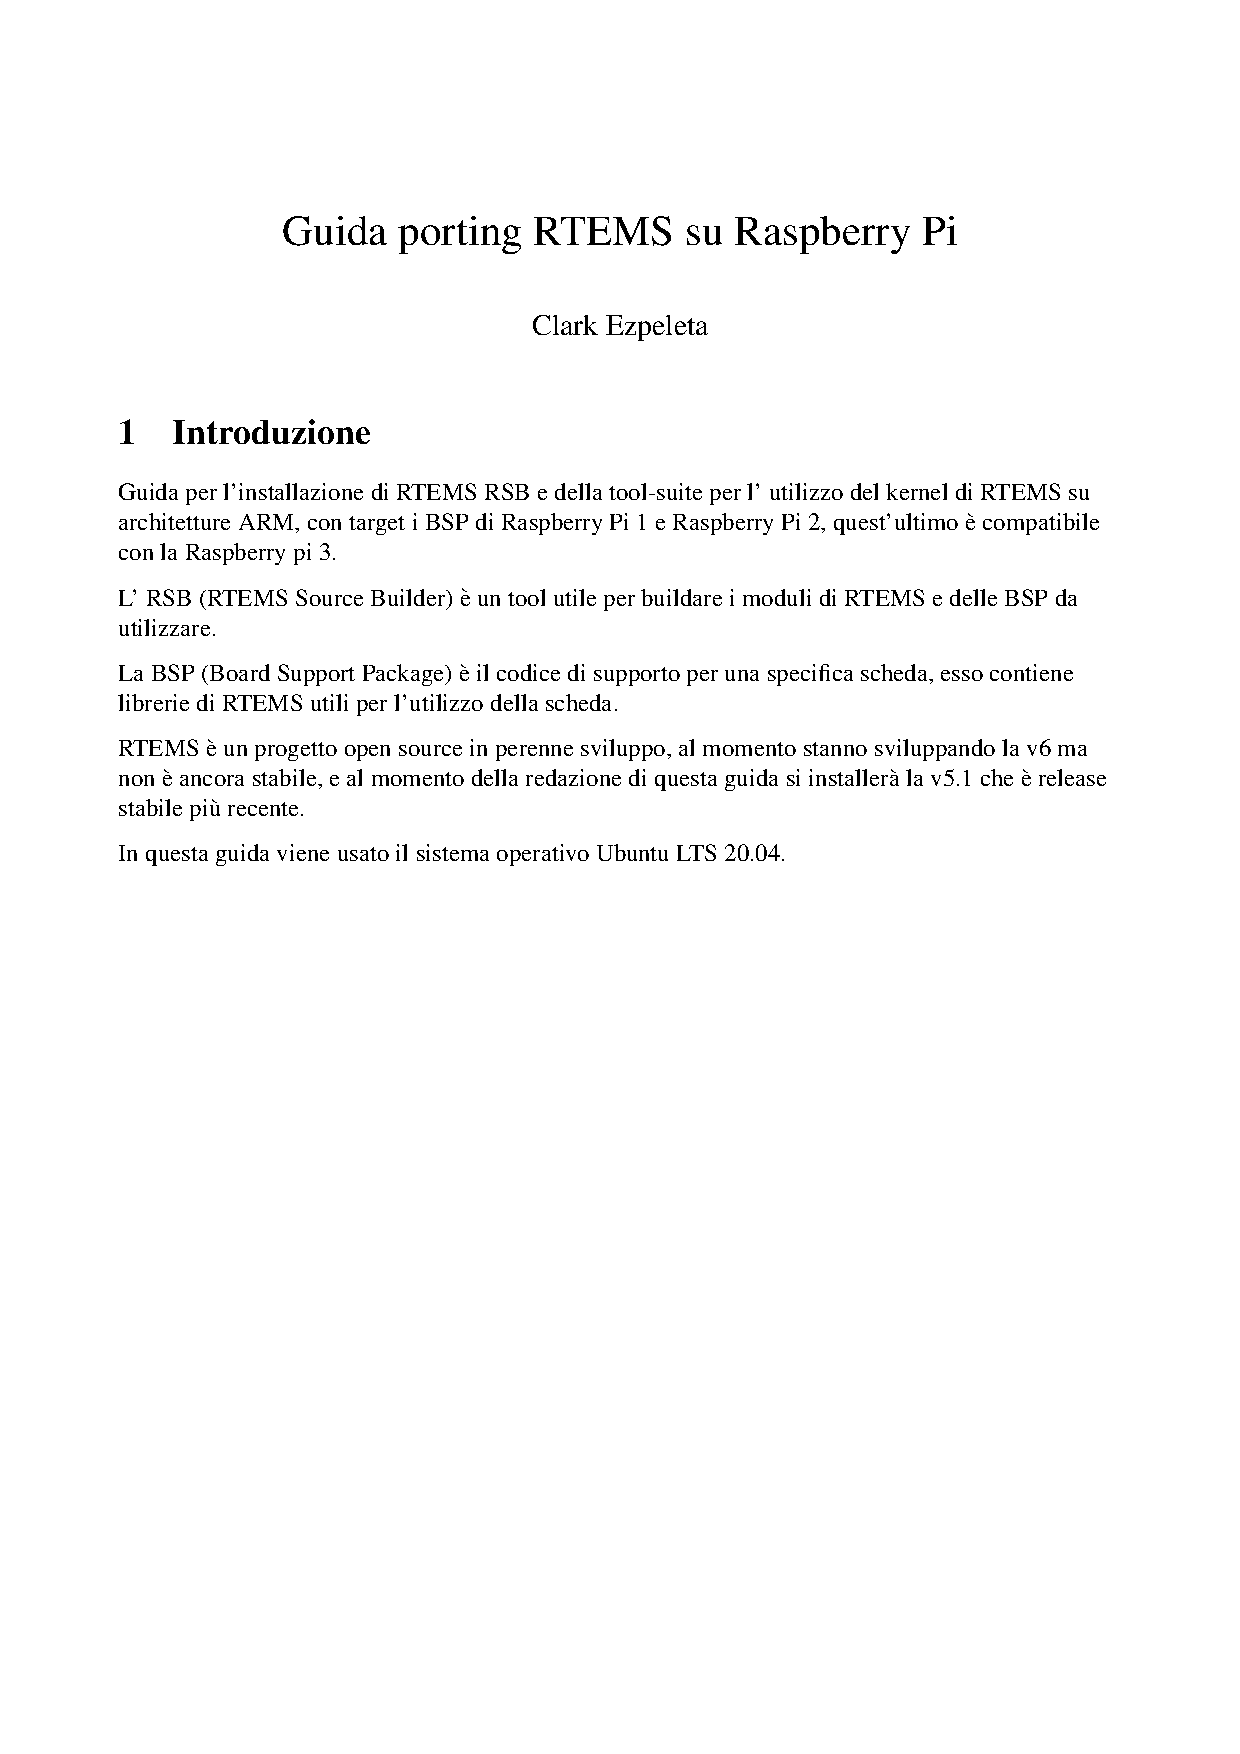
\includepdf[pages={-}]{Guida_porting_RTEMS.pdf}

\end{flushleft}

\end{document}
